\documentclass[12pt]{article}
\usepackage{graphicx}
\usepackage {color}
\usepackage{pdfpages}
\usepackage{float}
\usepackage{changebar}
\usepackage{enumitem,amssymb}
\renewcommand{\familydefault}{\sfdefault}
\usepackage[margin=1.2in]{geometry}
\usepackage{graphicx}
\usepackage{wrapfig}
\usepackage[super]{cite}
\usepackage{subcaption}
\usepackage[table]{xcolor}
\usepackage{amsmath}
\usepackage[sort, numbers]{natbib}

%%%%%%%%%%%%Defining the margins %%%%%%%%%%%%%%%%%%%%%
\textheight 9.in
\textwidth 6.5in
\topmargin -.5in
\oddsidemargin 0in
\setlength{\parskip}{\smallskipamount}

%%%%%%%%%%%%%%Specific Commands %%%%%%%%%%%%%%%%%%
\newcommand{\eg}{{\em e.g.,}}
\newcommand{\ie}{{\em i.e.,}}
\newcommand{\etc}{{\em etc.,}}
\newcommand{\etal}{{\em et al.}}
\newcommand{\degrees}{{$^{\circ}$}}
\newcommand{\fig}[1]{\textbf{Figure #1}}

%%%%%%%%%%%%%%%%%%%%%%%%%%%% Setting to control figure placement
% These determine the rules used to place floating objects like figures 
% They are only guides, but read the manual to see the effect of each.
\renewcommand{\topfraction}{.9}
\renewcommand{\bottomfraction}{.9}
\renewcommand{\textfraction}{.1}
\renewcommand{\familydefault}{\sfdefault} %setting the san serif font

%%%%%%%%%%%%%%%%%%%%%%%% Line spacing
% Use the following command for ``double'' spacing
%\setlength{\baselineskip}{1.2\baselineskip}
% and this one for an acceptable NIH spacing of 6lpi based on 11pt
%\setlength{\baselineskip}{.9\baselineskip}
% The baselineskip does not appear to work when we include a maketitle
% command in the main file.  Something there must set the line spacing
% If we use this next command, then things seem to work.
\renewcommand{\baselinestretch}{.9}

\setcounter{secnumdepth}{0} %make no numbers but have a table of contents


\begin{document}

\title{Lab 2, Ion Channel Simulations}
\author{Jake Bergquist, u6010393}
\maketitle
\tableofcontents
\newpage

\section{Introduction}
\par{}
While a larger goal of projects such as the Pysiome Project and the Virtual Physiological Human project are to develop tissue, organ, and system models for human Physiology, smaller scale models such as ion channel models are a vital part of these projects.\cite{Fink2011} Mathematical and computational models of Ion channels provide a framework for highly controlled investigation of the properties of these channels as well as the combination of vast amounts of experimental data into a single comprehensive model.  The modeling of ion channels contributes greatly to an effort to integrate and interpret experimental data as well as provide a highly detailed way to perform precise and otherwise technically impractical hypothesis testing on such a fine scale.
\par{}
While there are a vast variety of modeling techniques that range from basic current modeling with Hodgkin and Huxley to computationally intensive atomic scale molecular models, more frequently single ion channels are modeled using a Markovian chain of states model.\cite{Fink2011}\cite{Kojima2018a}
A Markovian model is one in which the next state of the model only depends on the current state, irrespective of the previous states. In the case of ion channels, Markovian models are typically structured into different closed and open states with rate constants that determine the probability of transitioning from one state to another. Each of these different states define different properties about the ion channel in the simulation, such as its permeability to ions, thus the effect on the conductance of those ions.\cite{Fink2011} In the most simple case of a two state Markovian ion channel model there is an open state and a closed state. At any given time the model may transition from closed to open or open to closed based on two rate constants, an open to closed rate, and a closed to open rate. If the closed to open rate constant were higher, this would describe a channel has a higher probability of being in the open state as opposed to the closed state. By increasing the number of states these models can be used to describe more complex behaviors such as channels with inactive states or drug/ligand binding that modulate activity. Each of these different state transitions have add rate coefficients describing the transitions between those states and other states, and thus a complex network can be built up.
\par{}
Each of the parameters that comprise the rate coefficients must be determined. Typically the values used come from direct experimental data from the channels of interest. This data includes structural information gained from crystallography, imaging data, genomic analysis, and perhaps most frequently from patch clamp electrical recordings. A patch clamp is a technique for assaying the electrical behavior of cells down to the single ion channel level. Either a specific cell expressing the channels of interest, such as a neuron or a cardiomyocyte, or a cell that has been made to express the channel of interest is isolated. A glass needle is used to either perforate or isolate a small section or patch of a cell membrane. In the case of perforation this allows access to the intracellular environment whereas in the case of isolation this allows access to the extracellular or intracellular membrane surface, depending on the preparation. In either case the concentrations of ions and other materials can be readily changed in the bath and within the needle. The voltage, injected current, or ion concentrations are then varied, and the resulting response of the ion channels can be measured via electrodes in the needle and extracellular space. Other parameters about the channels are derived from the structural information gained by crystallography and computational analysis given the amino acid sequence of the channels. These analyses are limited by the ability to isolate and crystallize the channels and the computation power and algorithms available to computer the atomic and amino acid scale interactions and models.
\par{}
As a result of years of work in this field on many different ion channels, vast amounts of data has been generated and funneled into constructing mathematical and computational models. The implementation of these models can often be difficult, however there are a variety of packages designed to incorporate the many different ion channel models into an centralized interface to allow for fast and robust testing of the models. Such libraries as CellML and applications like Jsim utilize these ionic models to allow researchers to perform robust simulations and tests with these models.
\par{}
In order to efficiently implement these various complex ion channel models, languages such as CellML have been developed. CellML is a markdown language built on top of XML as a way to standardize the development and sharing of models such as ion channel models. CellML allows researchers to easily share their models and parameters between different modeling environments, facilitating collaboration and distribution of developed models and findings. CellML itself is under active development and new improvements and tools are routinely implemented. Utilizing CellML as a standard language for writing models allows them to be easily shared and implemented in other settings. This significantly cuts down the time it takes to implement new models or test changes and additions to existing ones. Without a standard language like CellML the progress in developing and improving ion channel models would be hindered. For this lab we utilized Jsim as a simulation environment. Jsim is a java based simulation software developed by the Pysiome project for use in computational models and simulation based on experimental data.\cite{Fink2011} Jsim can read in CellML files and run the appropriate simulations, then display results in an interactive interface. Through Jsim, model parameters can be exposed for manipulation and testing, allowing for rapid and robust exploration of the model and effects of different parameters. Jsim allows for the testing of hypotheses and exploration of models in a lightweight, computationally inexpensive format that does not require significant experience or expertise with regards to developing CellML models.
\par{}
During this lab assignment we were required to simulate and manipulate membrane potential and ionic currents as well as a Markovian potassium channel model developed for a cardiac fibroblast.\cite{Sachse2008} Utilizing Jsim and the CellML cardiac fibroblast model developed by Dr. Frank Sachse we were able to explore the model and investigate the results from changing the different parameters such as ion conductances, stimulation protocols, and rate constants for the different Markovian states. Additionally the robust visualizations available through Jsim allowed for rapid visualization and interpretation of the model outputs and the effects of our changes and tests.

\section{Methods}
\subsection{1:Electrical Modeling of Membranes}
During this section we explored the relationship between the voltage at the membrane out our cardiac fibroblast and different stimulation protocols. Additionally we investigated the effects of ion currents on these membrane voltages.

\subsection{1.1}
\par{}
For the first investigation we loaded the fibroblast CellML model described in \cite{Sachse2008} and configured it to be a purely capacitive system. To do so we set all of the ionic and background conductances to zero. Specifically those parameters were the background conductance (Gb) the potassium conductance (Gkir) and the potassium shaker conductance (Pshkr). Next we set the stimulation to begin at 0.1 seconds with a duration of 1 second, an amplitude of 0.2 nA and a frequency of 1 Hz. The simulation was then ran for 6 seconds and the membrane voltage was plotted as a function of time. The system we have made here is a capacitor-current source system. 

\subsection{1.2}
\par{}
For the next section we took our purely capacitive cell from 1.1 and added a background (Gb) conductance of \ensuremath{1\times{}10^{-3}\mu S}. We also changed the reversal potential (Eb) to -84 mV. We then ran the same stimulation protocol as before with stimulation to begin at 0.1 seconds with a duration of 1 second, an amplitude of 0.2 nA and a frequency of 1 Hz. After 6 seconds of simulation we plotted membrane voltage, and membrane currents as a function of time. The system we created here is a resistor-capacitor system with a current source.

\subsection{2: Markovian Models of Ion Channels}
\par{}
During these next sections we manipulated the parameters of the potassium shaker channel Markov model present in the fibroblast model.

\subsection{2.1}
\par{}
First we adjusted the base fibroblast model to be capacitive and only have the potassium shaker current (Pshkr). The potassium (Gkir) conductance was set to 0, the background (Gb) conductance was set to zero, and the potassium shaker conductance was set to the default value of \ensuremath{5.4 \times{}10^{-9}\mu S}. The reversal potential was set to -85 mV and the stimulus was set to begin at 0.1 seconds with a duration of 1 second, and a frequency of 1 Hz. The amplitude of the stimulation was adjusted to cause a membrane voltage peak of +50 mV during the simulation. This value was found to be 0.55 nA. The simulation was run for 0.5 seconds, and the membrane voltage, as well as the Markovian states of all of the Pshkr ion channel model were plotted.

\subsection{2.2}
\par{}
We then took the model generated in 2.1 and modified it to delay the peak of the Pshkr O Markovian state by roughly 20 mS while maintaining a peak above 40\%. To do so we modified the values of the Markovian rate constants that dictated the transitions between the states. Specifically by lower the rate constants that dictated the transition between all of the closed states, as well as the closed to open states we could slow the progression through the states thereby delaying the opening peak. However, in order to make sure that the opening still had a significant peak value we needed to make sure to closed to open rate was sufficiently high to allow a quick state change once the model had reached that open to close transition, thereby allowing for a high peak for the open state.

\section{Results and Discussion}




\subsection{1.1}
\par{}
In figure \ref{fig:exp1.1} we see the results of the purely capacitive fibroblast with periodic stimulation. On the left in the figure we see the parameters used for this simulation and on the right we see the membrane voltage plotted as a function of time. As a result of setting all conductances to zero, thereby inhibiting any ionic or other current flow, we see that the membrane does not repolarize back to the starting or resting potentials as we might expect from a typical cell model. This demonstrates the necessity of some sort of conductance to be present in order for typical membrane repolarization to occur after a stimulus. Over the course of this simulation the membrane voltage steps incrementally from roughly -58 mV, (Which was set as the initial membrane potential) to roughly 200 mV in steps of roughly 50 mV. 

\begin{figure}[H]
	\centering
	\centering
	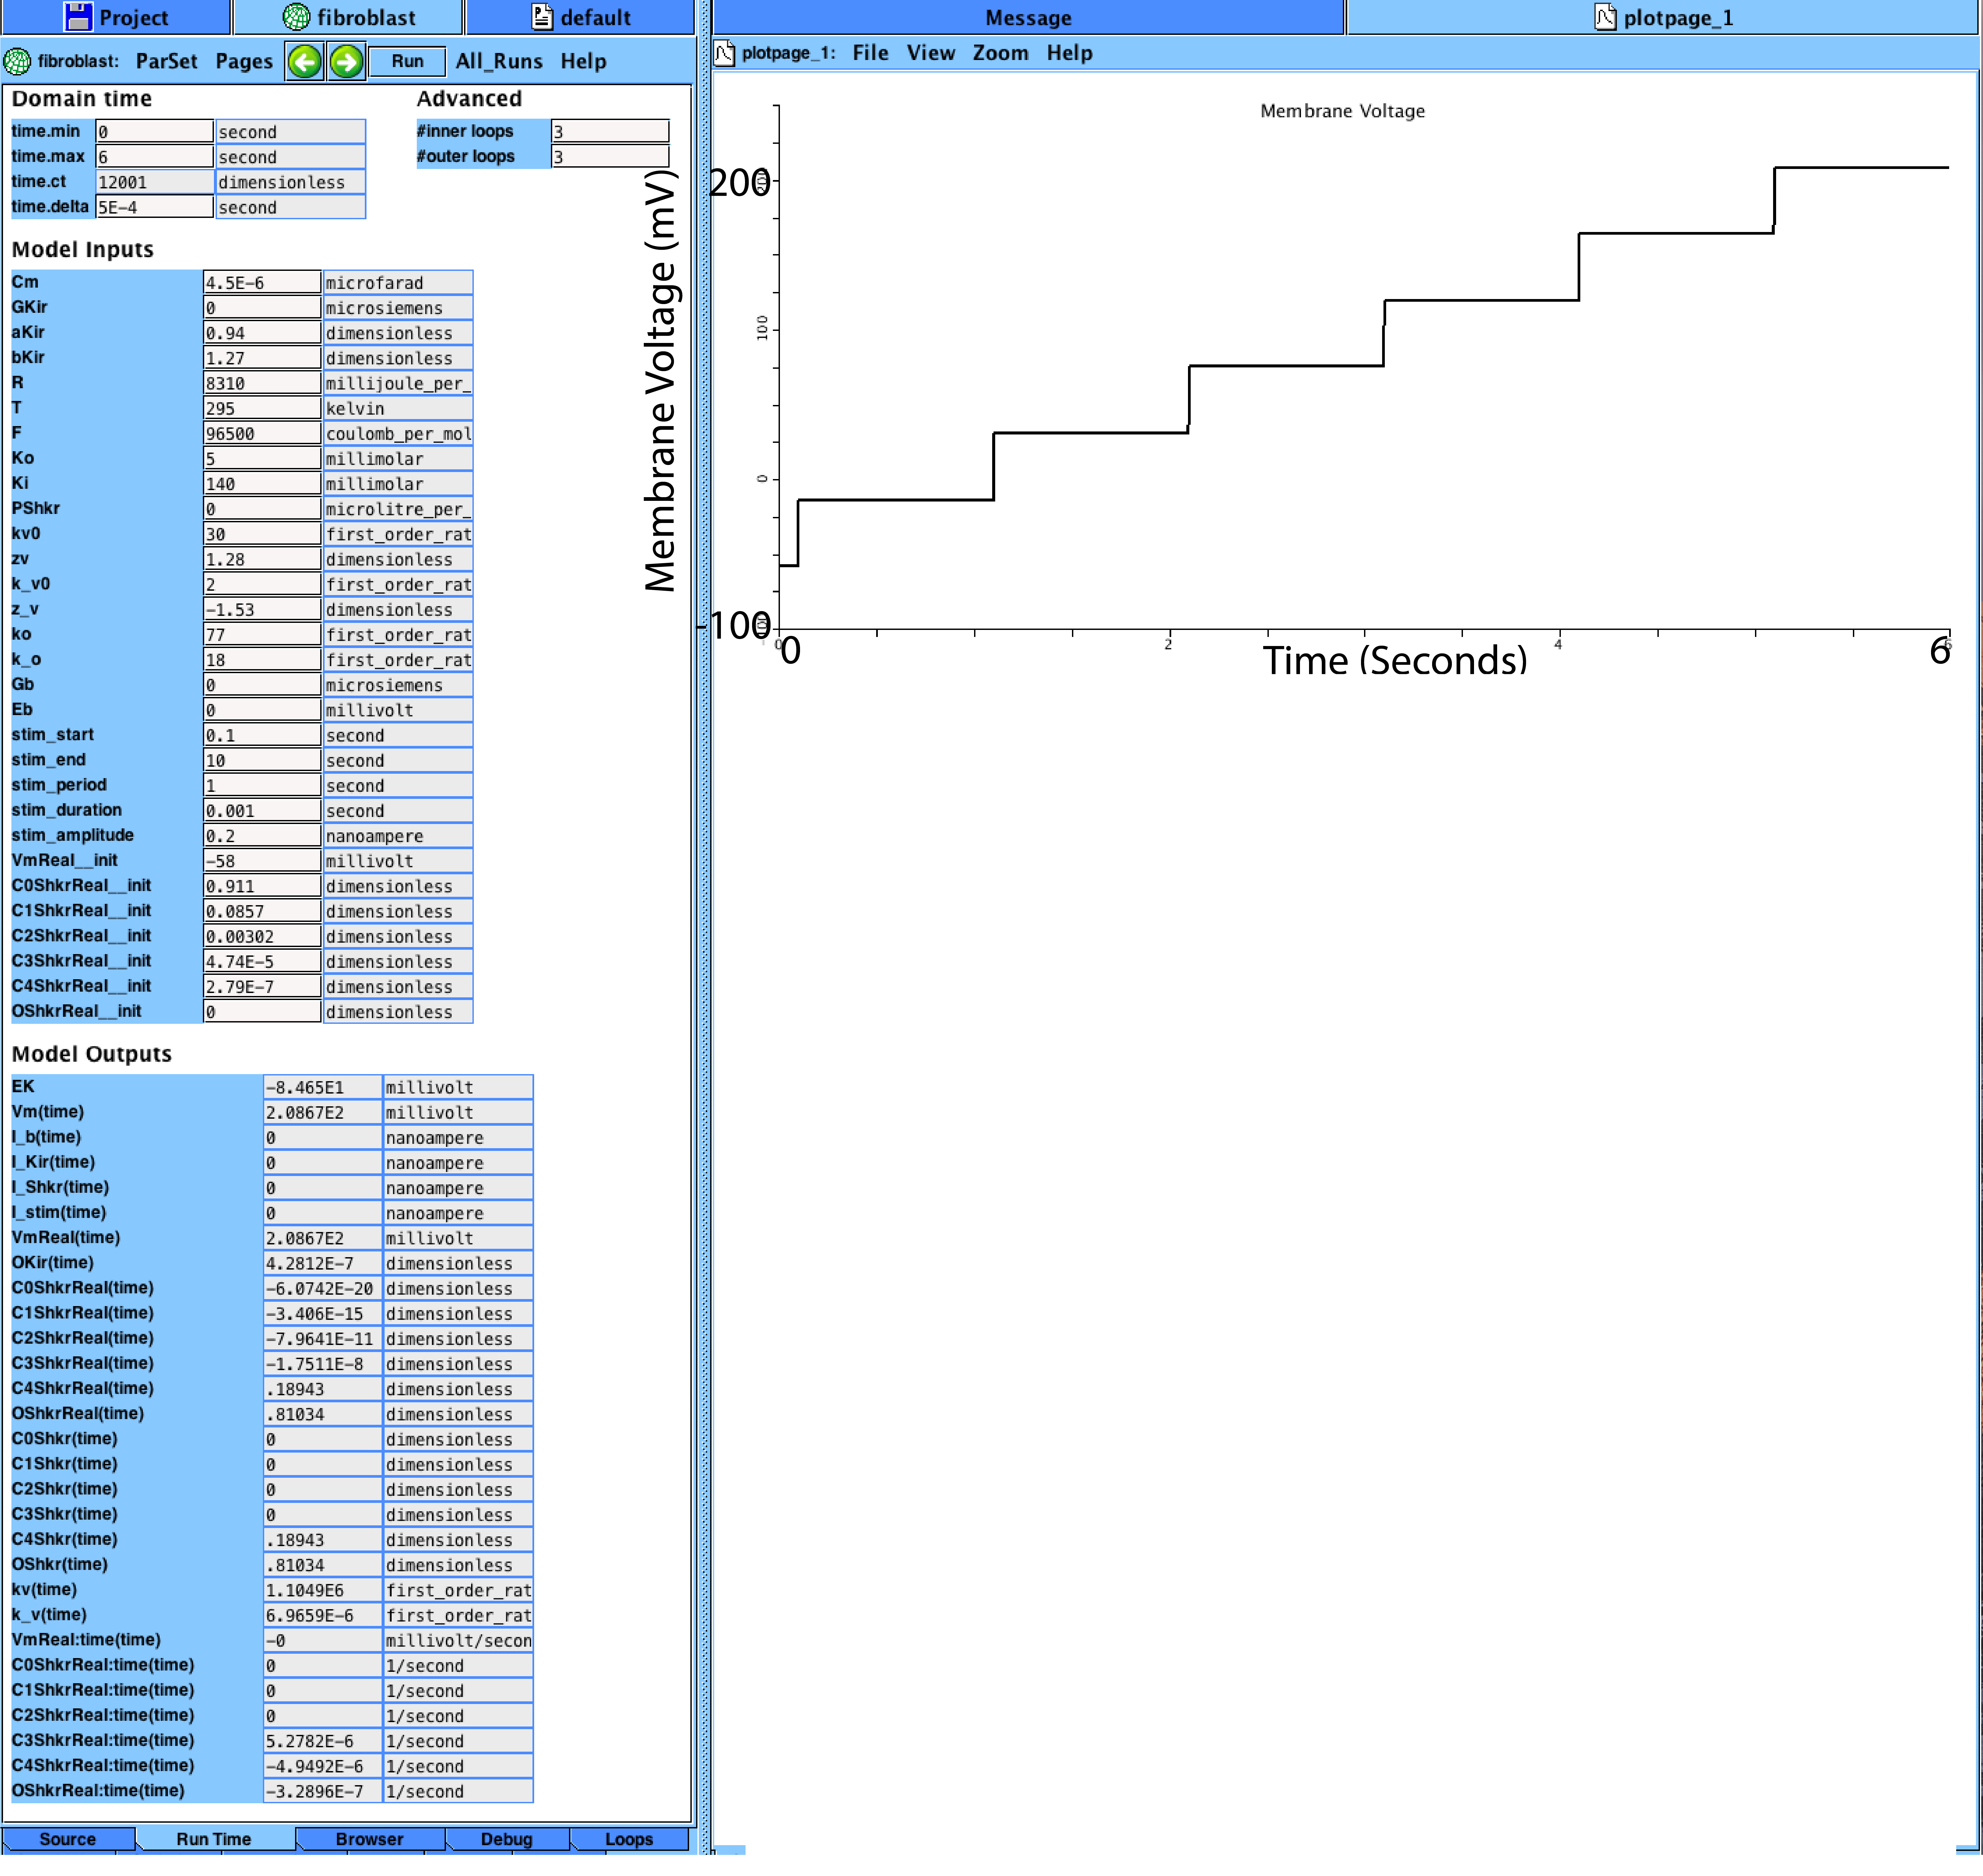
\includegraphics[width = .95\textwidth]{exp1.png}
	
	\caption{A screen capture of the parameters and output from Jsim for the first section. All conductances have been set to 0 \ensuremath{\mu} S and the stimulation protocol has been set according tot he methods. As can be seen the voltage incrementally steps from roughly -58 mV to roughly 200 mV. }
	\label{fig:exp1.1}
\end{figure}
\par{}
During this simulation we see that the membrane voltage (Vm) increases stepwise with each stimulus of injected current. This is because there are no ion channels present to allow for the current injected to flow across the membrane. By creating this purely capacitive system we are essentially only charging the capacitor with each stimulus, but not allowing any path for the accumulated charge to flow. Thus the membrane (or capacitor) voltage simply increases a fixed amount with each stimulation. Thus we can see from this experiment that the absence of any ion conductances, and therefor the absence of any functional ion channels in this membrane blocks the ability of the membrane to repolarize. The system we have created can be thought of schematically as described in figure \ref{fig:exp1.cmodel} wherein our current source charges a capacitor in short bursts but does not afford any path of discharge from the capacitor. In other words, when the current source is turned on (during our stimulu, according to the protocol) the capacitor charges. When the current source is off the capacitor does not charge, but because there is no path for the capacitor to discharged it sayes at the charge voltage from the previous stimulus. Now when the current source turns on it can charge the capacitor further.


\begin{figure}[H]
	\centering
	\centering
	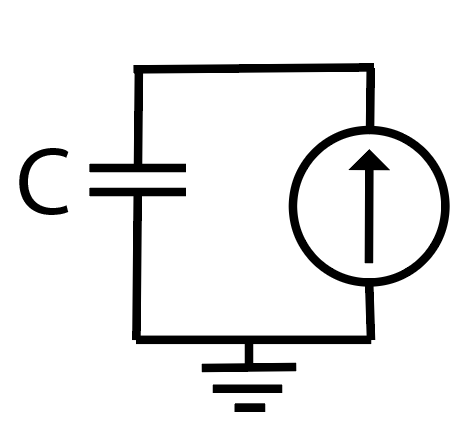
\includegraphics[width = .5\textwidth]{Capacitive.png}
	
	\caption{A circuit model of the simulation from 1.1. A current source provides energy to charge the capacitor C at a regular interval, but there is not path for the capacitor to discharge, thus the capacitor voltage will only increase with each successive injection of current from the current source. }
	\label{fig:exp1.cmodel}
\end{figure}	


\subsection{1.2}
\par{}
In figure \ref{fig:exp1.2} we see the input and output for 1.2. By taking the previously capacitive model from 1.1 and adding a background conductance of \ensuremath{1\times{}10^{-3}\mu S} we now see that the membrane voltage does not simply accumulate. Instead the membrane voltage jumps during the stimulation, but due to the background conductance, a current is allowed to pass through the membrane, allowing the membrane potential to repolarize back to the resting potential. The depolarization begins at 0.1 seconds (the onset of the first stimulus) and the repolarization completes by about 0.103 seconds. The peak voltage is roughly -74 mV, after which it returns to -84 mV.

\begin{figure}[H]
	\centering
	\centering
	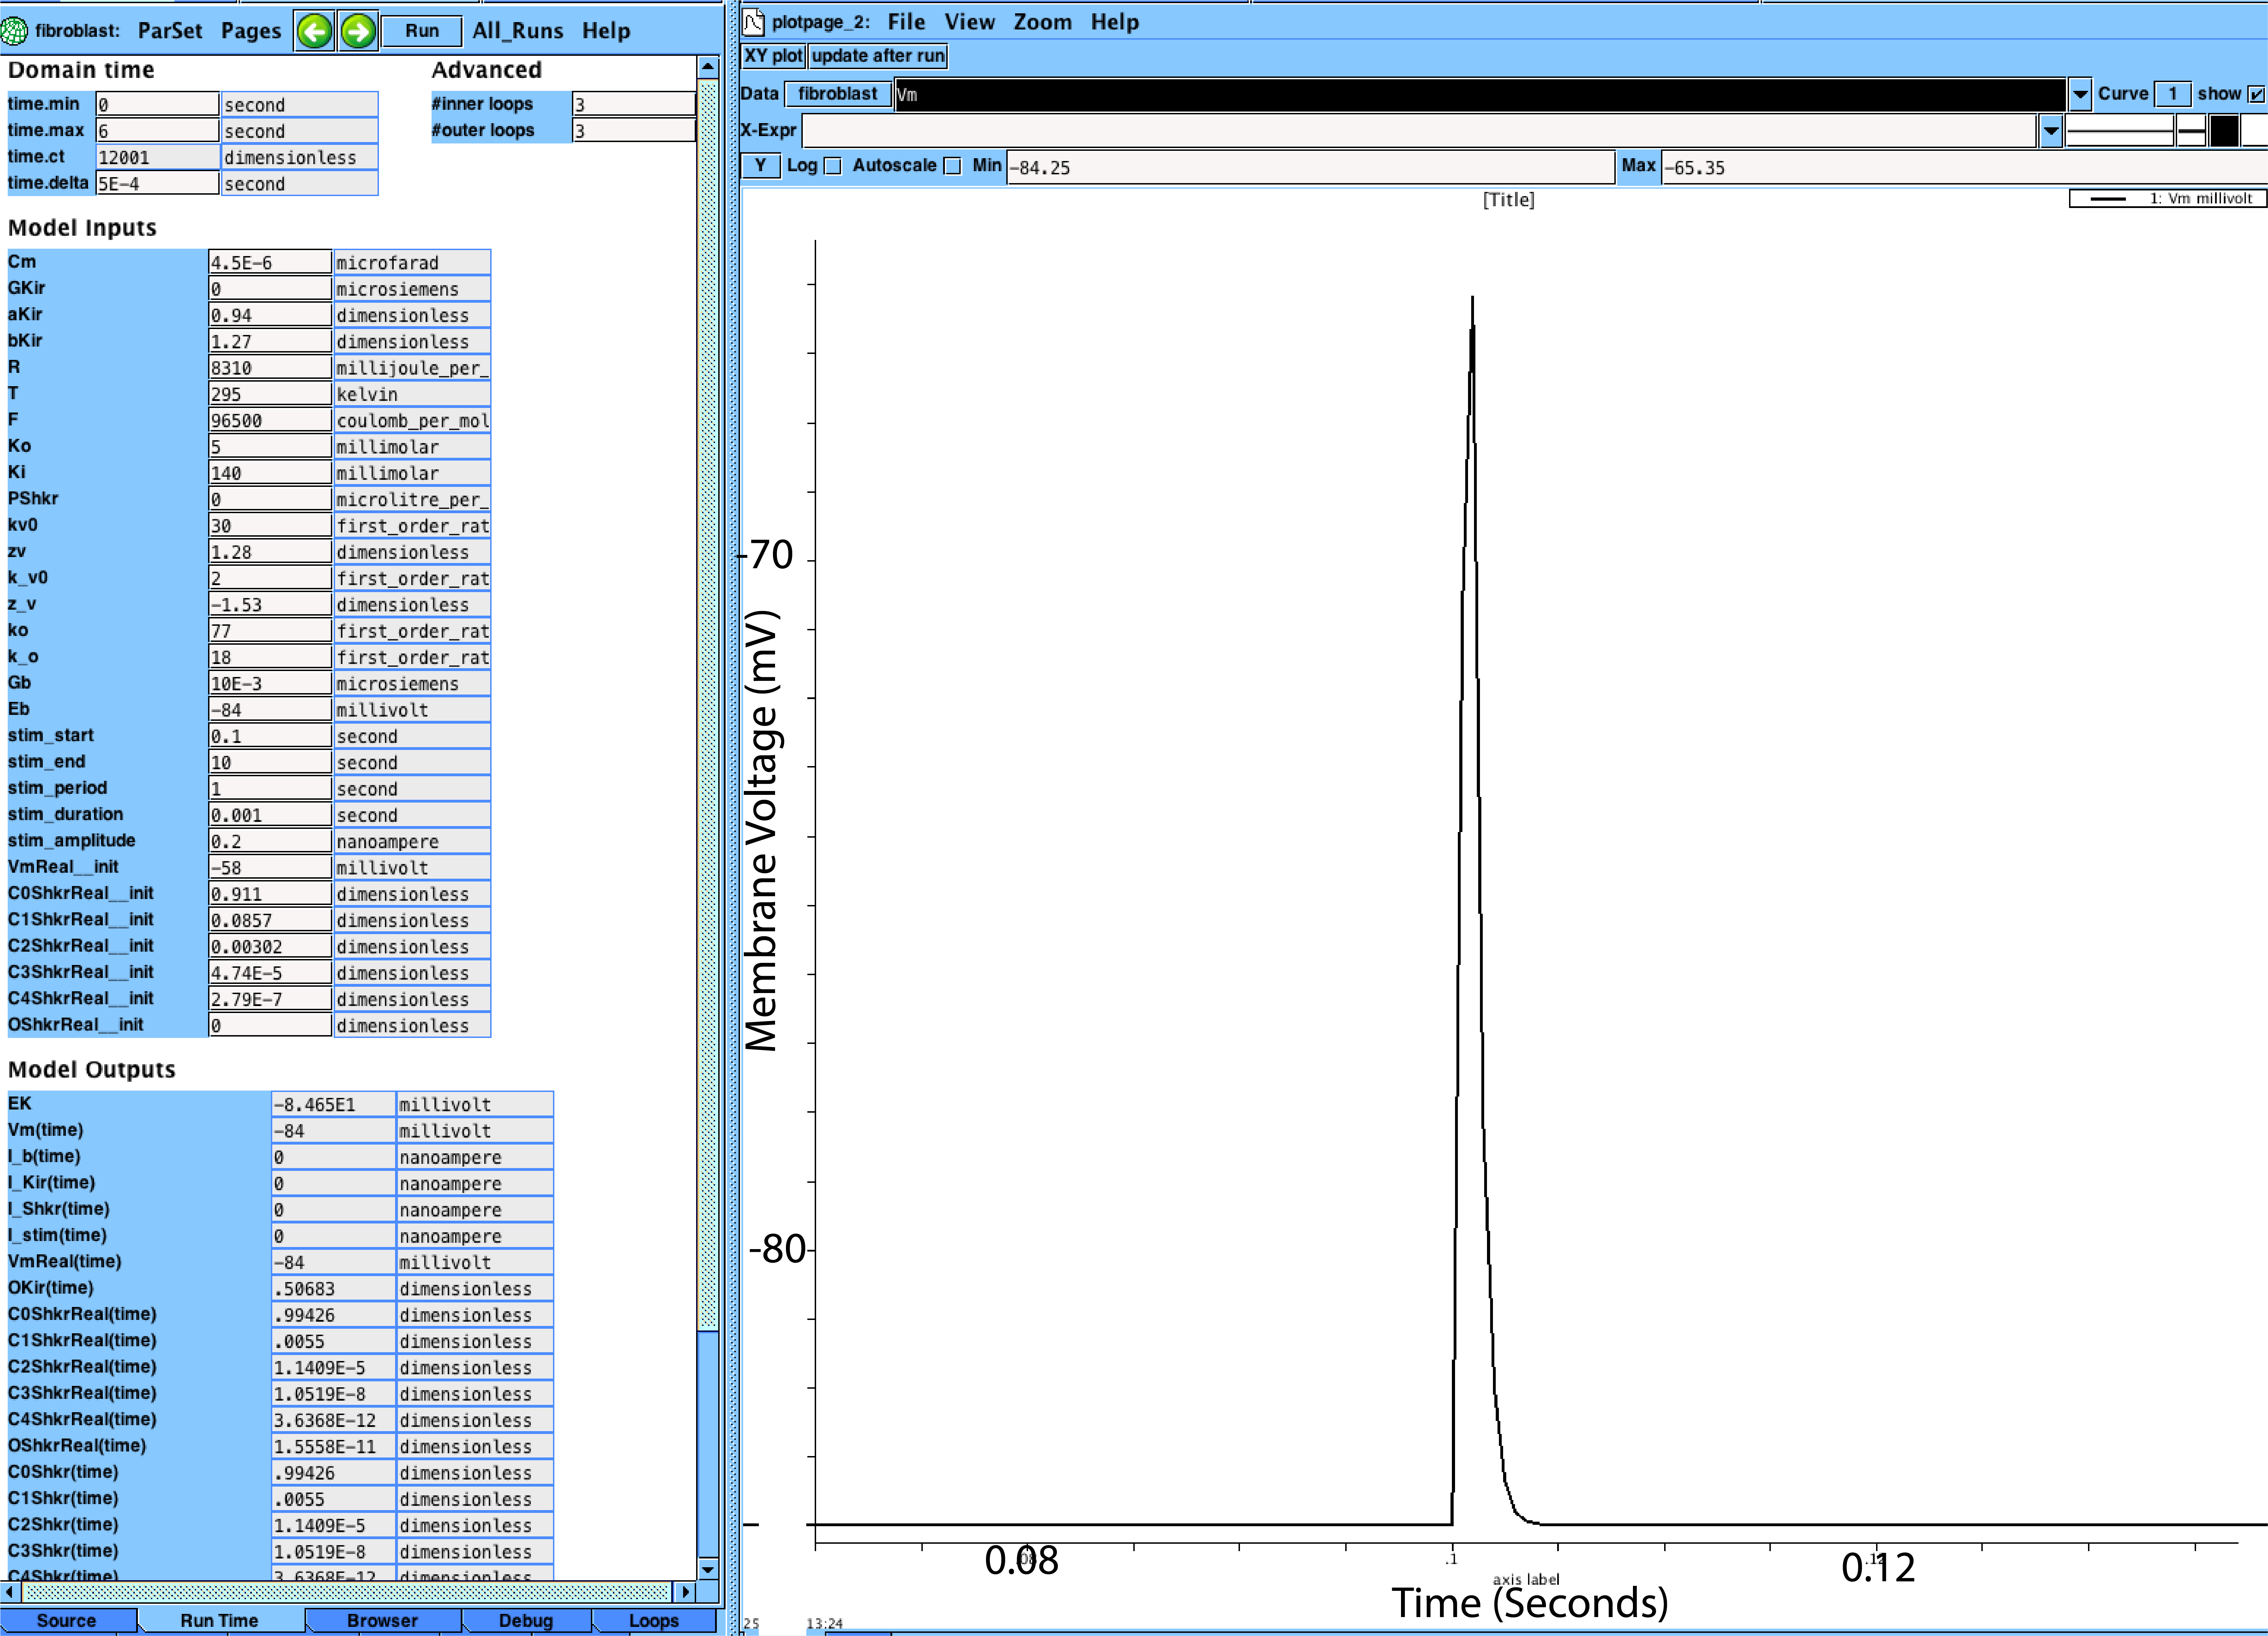
\includegraphics[width = .95\textwidth]{exp2.png}
	\caption{This figure shows the screen capture of the Jsim parameters and plotted membrane voltage for 1.2. Note that the Gkir and Pshkr conductances are set to 0 \ensuremath{\mu S}, the reversal potential (Eb) is set to -84 mV, and the background conductance (Gb) is set to \ensuremath{1\times{}10^{-3}\mu S}}.
	\label{fig:exp1.2}
\end{figure}

\par{}
The addition of the background current prevents the star stepping voltage we saw in 1.1. This is becuase we have given the voltage generated by the stimulus a path to discharge and repolarize via the background conductance. Thus our capcitor in our circuit model now has a method of discharge. This can be through of as adding a resistor in parallel with the capacitor, as seen in figure \ref{fig:exp1.rc}. The current source charges the capacitor when it is on (additionally while the current source is on, during stimulus, some current flows through the resistor, additionally the voltage on the capacitor during each stimulus is partly deterined by the resitance of the resistor, which is why we see a lesser voltage jump as compared to that seen in figure \ref{fig:exp1.1}). When the current source is off we now have a capacitor charged to some voltage in parallel with a resistor. This provides a path of discharge for the capacitor through the resistor. The rate of discharge can be seen in the sloped discharge in figure \ref{fig:exp1.2} and can be calculated via equation \ref{eq:rc}. The value of that resistor is 1/Gb $\Omega$, thus in this case 1 K$\Omega$. 

\begin{figure}[H]
	\centering
	\centering
	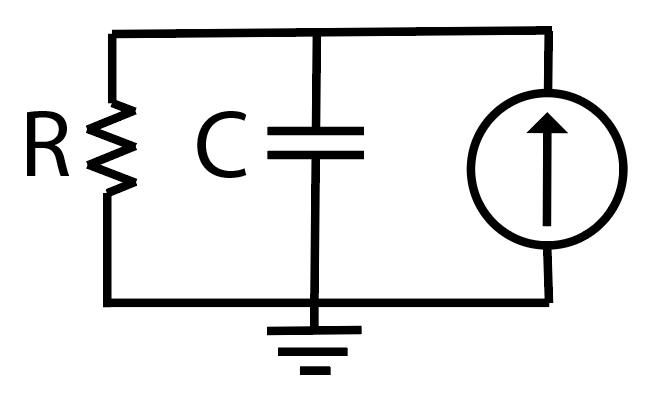
\includegraphics[width = .95\textwidth]{RC.png}
	\caption{A circuit model for the simulation in 1.2. A current source provides energy to charge the capacitor C. The resistor R allows current to flow both during stimulus and after. When the current source is not providing stimulus the capacitor discharges through the resistor. The resistor represents the background conductance through the membrane while the capacitor represents the capacitance of the cell membrane}.
	\label{fig:exp1.rc}
\end{figure}

\begin{equation} 
V(t) = V_0 e^{t/RC} 
\label{eq:rc}
\end{equation}

\subsection{2.1}
\par{}

During this section we worked with the Markovian ion channel model for the time and voltage dependent outward current Ishkr, presented in \cite{Sachse2008}, and shown in figure \ref{fig:markModel}. In this model we can see that there are five closed states, labeled C0 - C4, and one open state labeled O. The rate constants between each state are shown in figure \ref{fig:markModel}. Of particular note is that the rate constants between each closed state are all derived from the same values. K\textsubscript{V} is used for all of the forward rates while K\textsubscript{-V} is used for all the reverse rates. The goal of this first section was to configure the fibroblast to be only capacitive in addition to the Ishkr current. To do so, Gb, and Kir were set to 0 \ensuremath{\mu S}. Additionally Eb was set to -84 mV and the stimulus protocol was set the same as before. We then had to adjust the stimulus amplitude to result in a peak membrane voltage of +50 mV. To do so we adjusted the amplitude to 0.55 nA as seen in figure \ref{fig:exp2.1mv}. This resulted in a membrane voltage peak of just over +50 mV. 

\begin{figure}[H]
	\centering
	\centering
	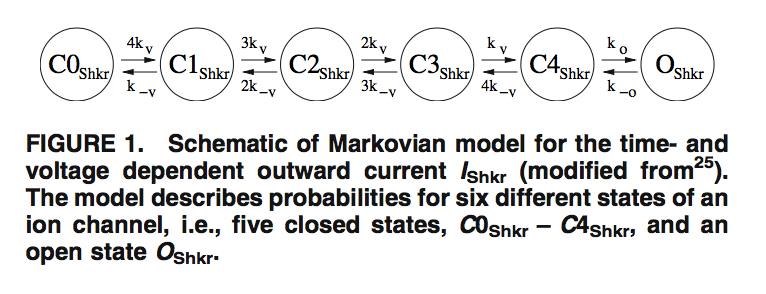
\includegraphics[width = .95\textwidth]{markovfig.png}
	
	\caption{ This figure shows the markov model used for modeling the kshaker channel for these simulations. Figure sourced from \cite{Sachse2008}}
	\label{fig:markModel}
\end{figure}

\begin{figure}[H]
	\centering
	\centering
	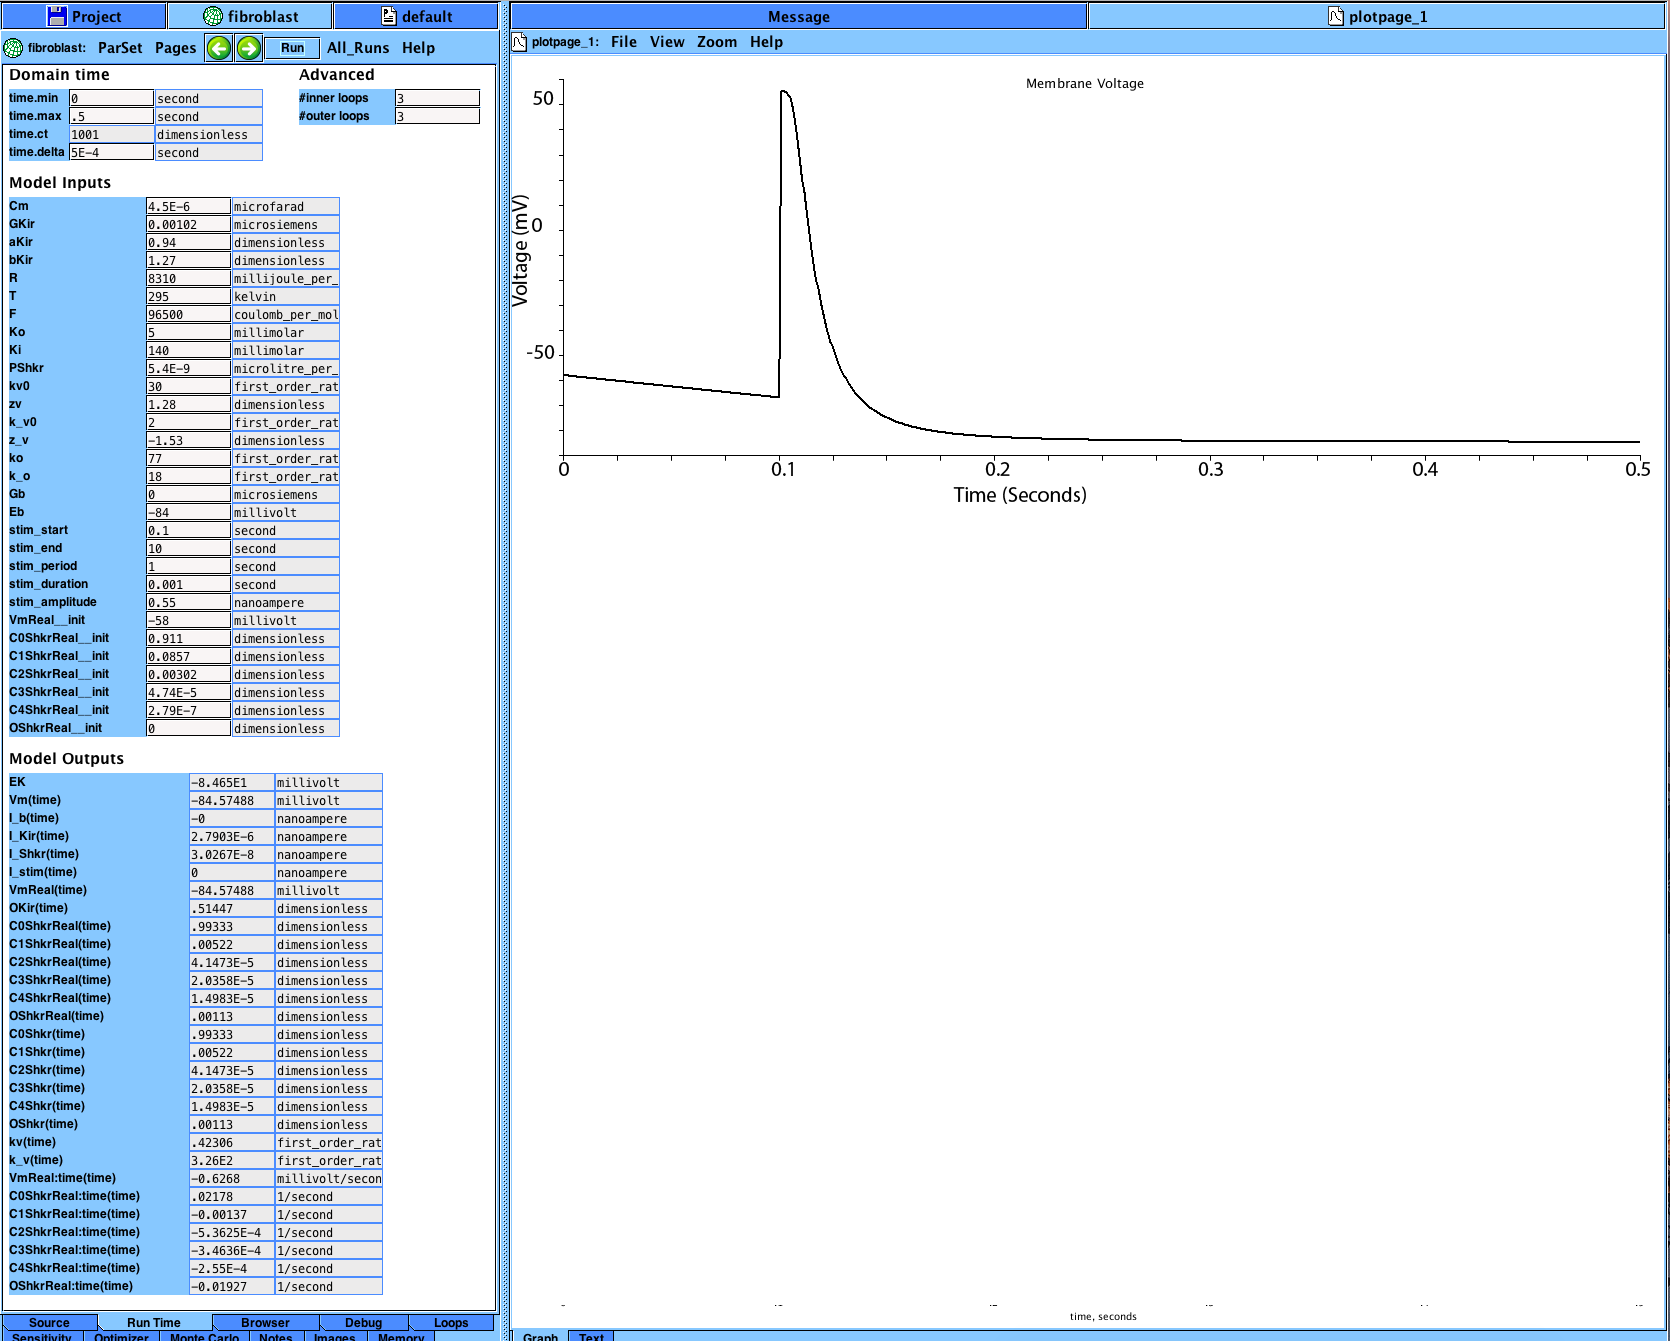
\includegraphics[width = .95\textwidth]{Exp3mv.png}
	
	\caption{ This figure shows the Jsim parameters and plotted membrane voltage as a function of time for 2.1. As can be seen the stimulus amplitude has been raised to 0.55 nA, resulting in a membrane peak above +50 mV.}
	\label{fig:exp2.1mv}
\end{figure}
\par{}
We then plotted the probability states for each of the Markvoian states, which can be seen in figure \ref{fig:exp2.1}. As expected the probabilities are such that at the beginning the C0 probability is the highest, meaning the model is likely in the C0 state before stimulus. What is interesting however is that C0, C1, C2, and C3 are all bimodal, whereas C4, and O are not. This is curious given the linear Markovian model of this ion channel (figure \ref{fig:markModel}). However if we look more closely we can see why this is the case. The model begins in C0, then as the voltage jumps the C1 probability goes up, representing a state change to C1. The same is true for C2, C3, and C4 in that order. It already is clear why the O state is not bimodal, as we only stay in this state once, however we would expect all the closed states to be bimodal as we must transition back through them to get back to the C0 state. Why then is C4 not bimodal? To explain this we must look closely at the rate constants. For the C0 to C1 transition the rate is 4K\textsubscript{V} but from C1 to C2 it is 3K\textsubscript{v}, then 2K\textsubscript{V} for C2 to C3 and K\textsubscript{V} for C3 to C0. So we see that the transitions as we go through the states from C0 to C4 are slowing down. Indeed we see that the first peak of the C1 probability is very narrow (red line in figure \ref{fig:exp2.1}) as the model passes into C1 and then to C2 almost immediately. However in the other direction the opposite is true. The rate constants going from C4 back towards C0 decrease. Thus the transition from C4 to C3 is much faster than C3 to C2 and so on. Additionally the rate constant between C4 to O is very high while the rate constant from O to C4 is lower by comparson (77 and 18 respectivly, unitless constants). Thus as the model progresses back from O through the C states the probability of staying in the C4 state is very low as both rate constants to exit that state are relatively high. Thus there is only one peak for this state. As we progress back toward C0 from C4 the other state transitions are slower in that direction, with the added factor that the rate constant to go in revers (\ie back towards C4) are also slow as previously discussed. Thus for the C3, C2, and C1 states there is another peak where the probability of being in that state is high again for a short time. The C0 state is biomodal simply because it is the resting state to which the model returns.

\begin{figure}[H]
	\centering
	\centering
	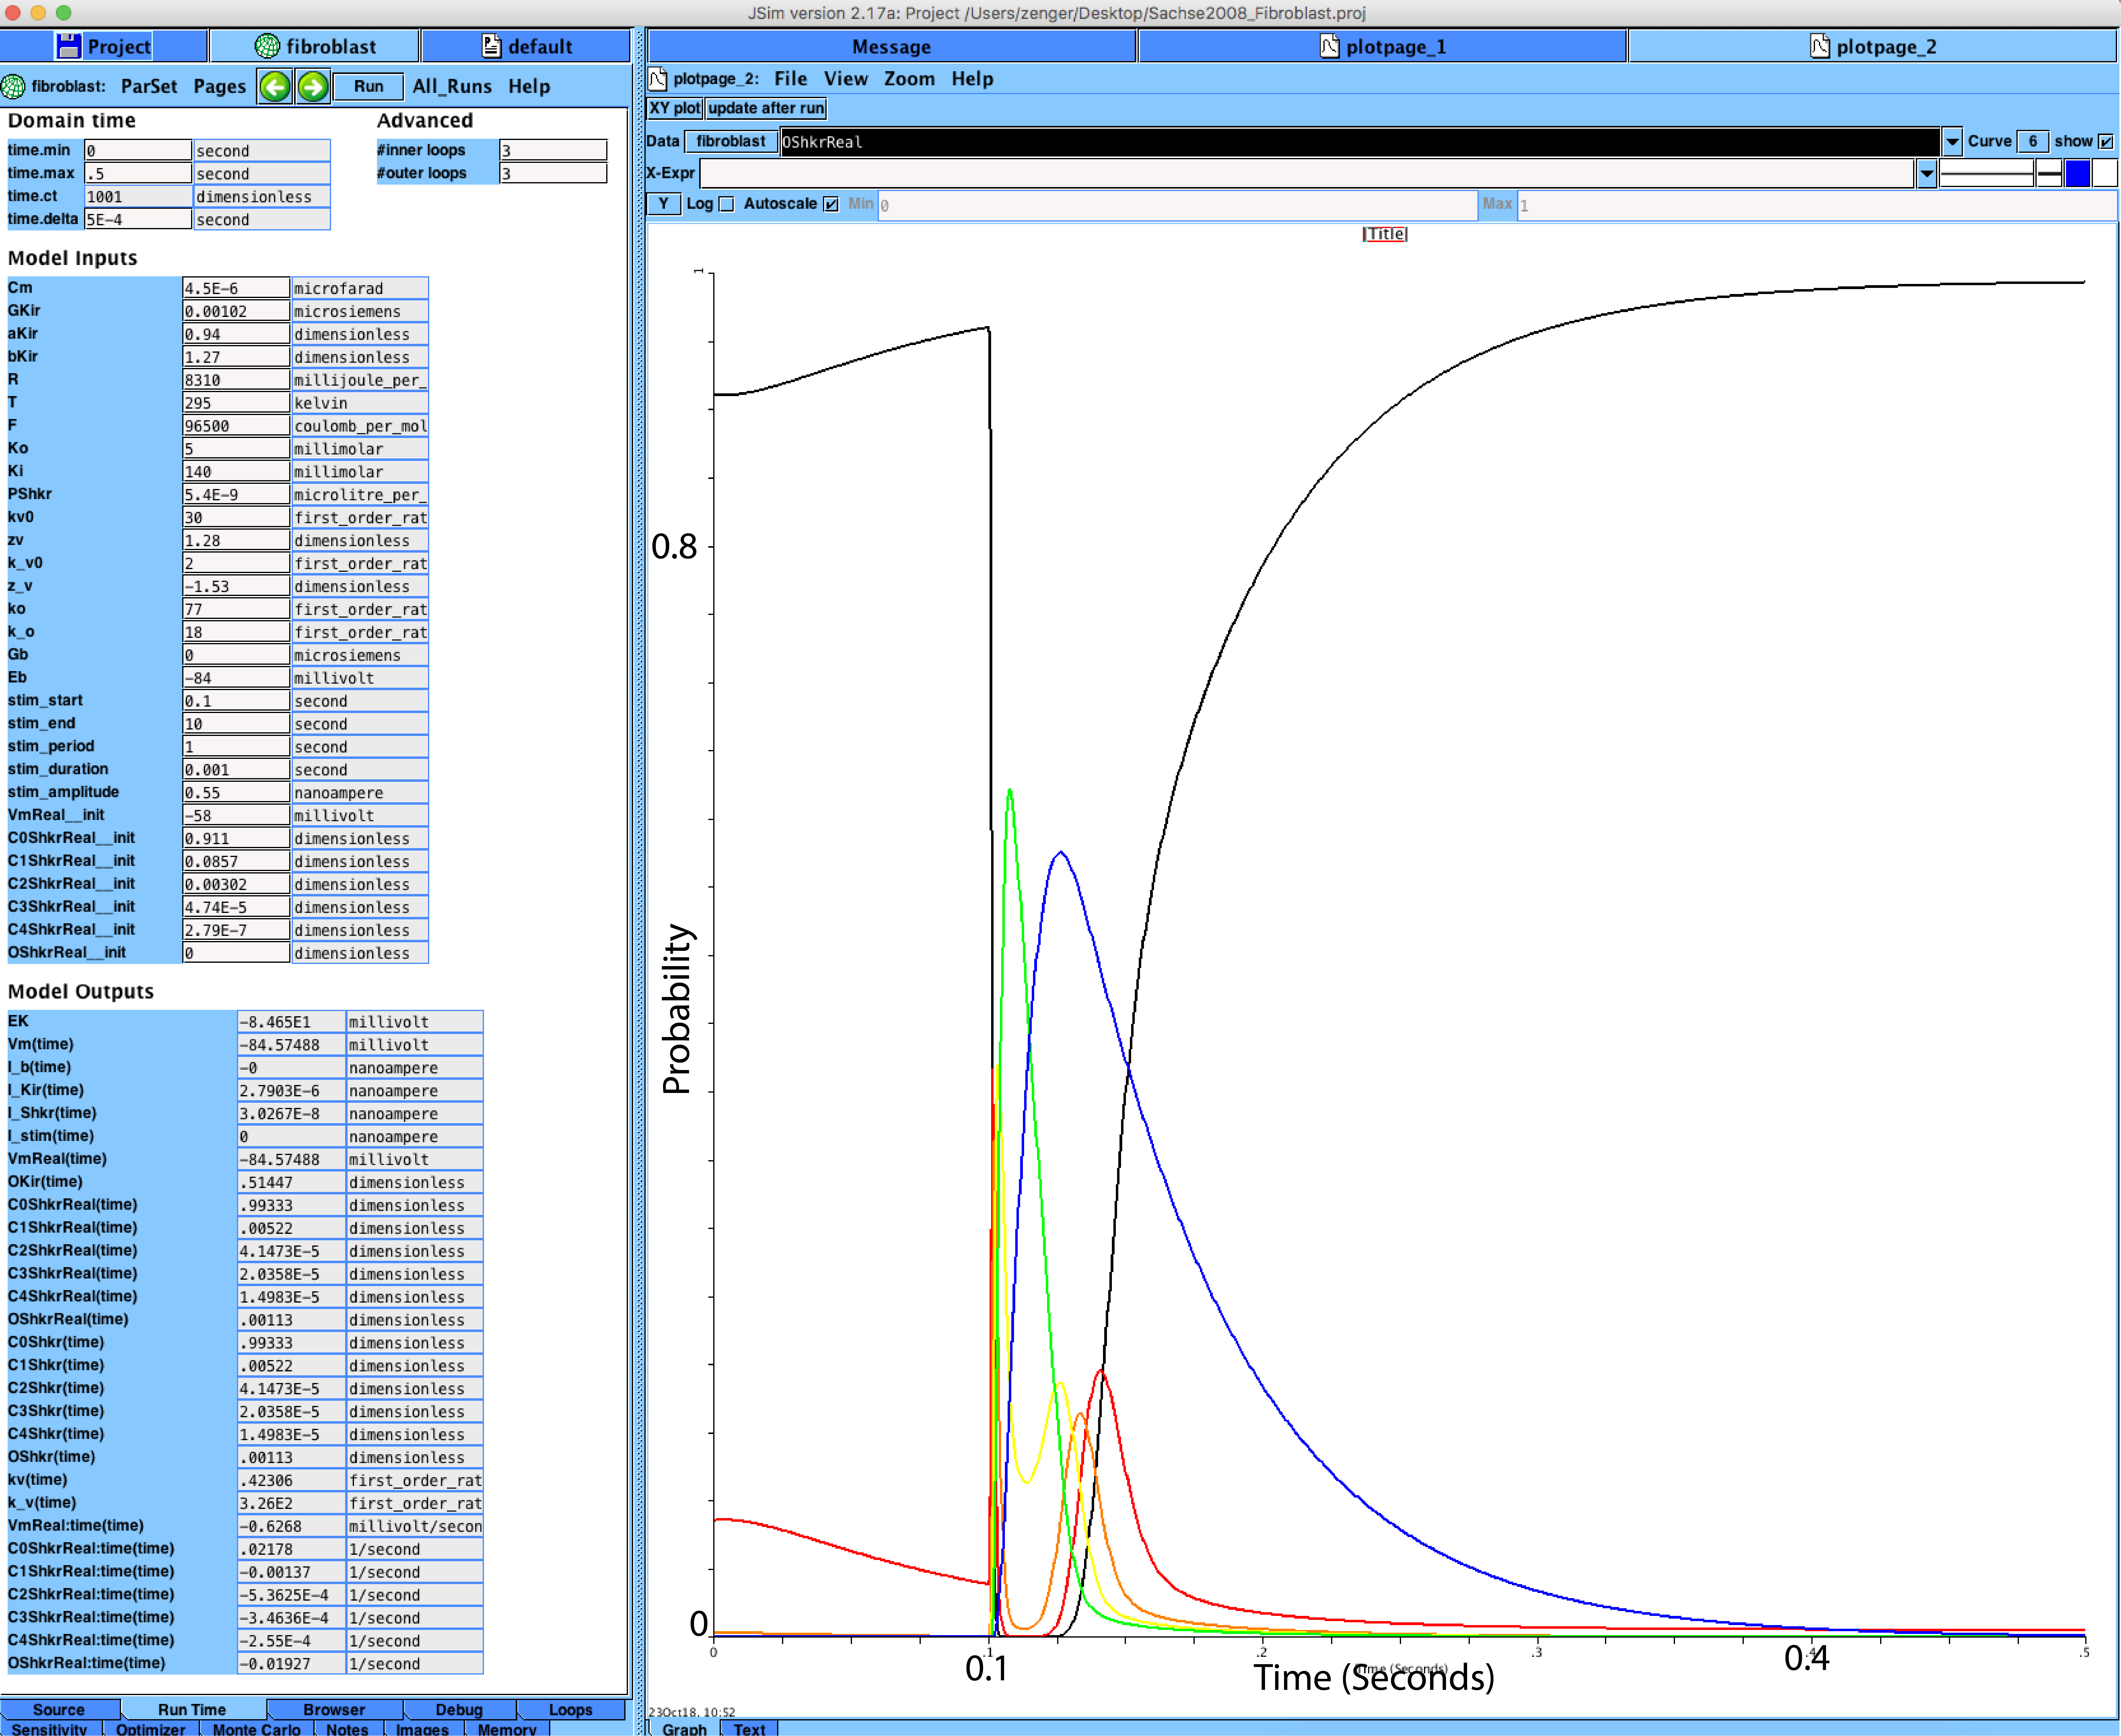
\includegraphics[width = .95\textwidth]{exp3.png}
	
	\caption{ This figure shows the markov probabilities for each state represented in the model during our described stimulation protocol. This is for the Kshaker channel only. The black line is C0Shkr, the red line is C1Shkr, the orange line is C2Shkr, the yellow line is C3Shkr, the green line is C4Shkr, the blue line is Oshkr.}
	\label{fig:exp2.1}
\end{figure}


\subsection{2.2}
\par{}
In this section we manipulated the rate constants to delay the O state peak by roughly 20 mS without having the peak value drop below 40\%. We first attempted to lower the k\textsubscript{O} constant to delay the C4 to O transition, however doing so also severely lowers the O peak. However decreasing k\textsubscript{v} delays the transitions between the C states towards the O state, thereby delaying the O peak. After iteratively manipulating these parameters we came to a final parameter set where k\textsubscript{v} (Kvo) was changed from 30 to 20, k\textsubscript{O} was changed from 77 to 30, and k\textsubscript{-v} (k-vo) was changed from 2 to 0.5. Figure \ref{fig:exp2.2} shows the resultant shift in the peaks. As can be seen we achieved a 20-25 mS delay in the O peak (blue line) without decreasing the peak below 40\% as compared to figure \ref{fig:exp2.1}. 
\begin{figure}[H]
	\centering
	\centering
	\includegraphics[width = .95\textwidth]{exp4.png}
	\caption{  }
	\label{fig:exp2.2}
\end{figure}



\section{Conclusions}
\par{}

The power of CellML as a modeling language is that it allows for quick and robust generation of easy to work with models such as the one explored in this lab. This becomes especially apparent when we consider how easily generated models can be shared, modified, and accessed by collaborators and other researchers through a variety of simulation software. As an language in active development it is constantly being improved and added to by a large community. At this point there are models for many different ion channels and entire cells that can easily be combined and accessed. By standardizing the way in which these models are developed a large barrier between collaborators is removed and progression and development of models is not hindered by differences in model format. Additionally, a disadvantage of models, being that they can become obsolete as new ones are developed, is mitigated by the easily shareable nature of CellML models. New models can rapidly be dispersed and tested by others as well as incorporated. If a model we were using became outdated it would be easy to incorporate the update CellML directly into our simulation software with minimal effort.
\par{}
Simulations are a diverse tool that allow for the assembly of data from many different sources into a cohesive structure that reflects many aspects of observed physical phenomena. Additionally simulations provide an advantage of a flexible base for hypothesis testing that would not be feasible via traditional means. If a researcher wanted to test changing the concentrations of an ion outside of the cellular membrane by increments of 1 uM this would be exceedingly arduous and time consuming in an in virto set up. However with a model of the cell in question and a computer and simulation software (such as Jsim) that researcher could feasibly perform such a hypothesis test in a matter of minutes to hours. The amount of fine tuned control over a wide variety of variables is unrivaled in simulations by traditional methods. However there are noteworthy drawbacks. A common saying is that all models are wrong, some models are useful. That is to say, a model may be good for describing the actual phenomena in one circumstance, but completely wrong in a different setting. Thus care must be taken when designing models and selecting one for specific tests. Additionally a model can only be as good as the data and formulations that are used to create it. As new data is being uncovered by more traditional methods, models must constantly be improved. Therefore it is unlikely that models and simulations will ever really replace all of the scientific inquiry process. That being said, models can serve as excellent tools to guide research. Testing initial ideas in a model can give direction to more specific research in vitro. 
\par{}
Models also serve a more translational purpose. One goal of the pysiome project is to be able to generate a patient specific model for all organ systems. Such a tool would allow clinicians to identify effective treatment plans and better predict treatment outcomes and complications. Models such as the ones we investigated in this lab can also be used to test the effects of drugs and disease states in these settings. These findings can then be used as inputs for pharmacological studies on drug formulation and treatment plans. 
\par{}
In the end, given the current state of the art, models cannot replace direct experimentation. There are many factors that models do not account for which can currently only be accessed by direct experiments. For example, given how the model we used today is structured, we woudl not be able to test the effects of an novel compound on the membrane currents of our fibroblast model. However more sophisticated models are constantly being built. Such models could even predict the effects of such a novel drug if the model were formulated to account for the structure of the proteins of interest and their various interactions. Overall no model is complete, and in order to better fill them out researchers must constantly work to develop, validate, and add experimental backing to the models. Having a model that is sophisticated is not the only factor as well. The model must also be feasible to process on a computer. While there are more and more advanced super computers capable of nearly unimaginable levels of calculations, there are still some models too complex to be usable. Thus a constant constrain on a model is for it to be usably simple, but sufficiently complex to accurately  describe a phenomena.
\par{}
Overall our experience in this lab showed us the robust flexibility of using models for scientific inquiry. We were able to rapidly and easily test the effects of different parameter alterations on the response of the model cell. This worked well not only as teaching tool for us to understand the underlying physiological principles but also as a method of hypothesis exploration and testing. Simulations are rapidly gaining popularity in the scientific community for their ease of use and robust nature. As the scientific community proceeds we must be vigilant to continually validate and improve our models, and ensure we are selecting appropriate models for the tasks at hand while recognizing and working within the limitations of our modeling framework with respect to the conclusions we draw from them. The CellML project has provided an excellent method of unifying the model development to allow for more robust collaboration and easier dissemination and application of models within the modeling community. That combined with simulation tools like Jsim will drive simulation based research forward.

%%%%%%%%%%%%%%%%%% Correct Bibliography Style

\bibliography{C:/Users/Jake/Documents/library}
\bibliographystyle{IEEEtran}


\end{document}


%%%%%%%%%%%%%%%% Table Example %%%%%%%%%%%%%%%%%%%%%%
\rowcolors{2}{gray!25}{white}
\begin{table}[H]
	\centering
	\caption{Simulated measurements for conduction velocity and maximal upstroke velocity}
	\label{tab:results}
\begin{tabular}{ccc}
	\hline \hline
	Experiment  & Conduction Velocity & Maximal Upstroke Velocity\\ 
	Number & (cm/ms)& (mV/ms) \\
	\hline
	 1 & 16.6389 &  69.8933 \\ 
	 2 &  18.9606&  73.9121 \\ 

	 3 &  24.7062&  83.871 \\ 

	  4&  45.2948&  109.1537\\ 

	  5&  52.6004&  116.8785\\ 

	  6&  77.6482&  131.6630\\ 

	  7&  2.0641&  0.0222\\ 

	  8&  44.0706&  109.3527\\ 

	  9&  45.2948&  109.1675\\ 

	  10&  2.1013&  -0.0024\\ 

	  11&  2.0896&  -0.0024\\ 

	  12&  60.3930&  179.3235\\ 
	  13&  38.8214&  86.8933 \\ 

	  14&  31.9728&  60.6956\\ 

	  15&  27.6375&  48.7076\\ 
	  16&  23.2945&  35.4873\\ 
	  17&  20.3827&  28.0958\\ 
	\hline 
	\hline
\end{tabular} 
\end{table}

%%%%%%%%%%%%%%%%% Figure Example %%%%%%%%%%%%%%%%%%%
	\begin{figure}[H]
	\centering
	\begin{subfigure}{0.49\textwidth}
		\centering
		\includegraphics[width = \textwidth]{../Simulation/Experiment_11.png}
		\caption{}
		\label{fig:left}
	\end{subfigure}
	\begin{subfigure}{0.49\textwidth}
		\centering
		\includegraphics[width = \textwidth]{../Simulation/Experiment_9.png}
		\caption{}
		\label{fig:right}
	\end{subfigure}
	\vskip\baselineskip
	\begin{subfigure}{0.49\textwidth}
		\centering
		\includegraphics[width = \textwidth]{../Simulation/Experiment_4.png}
		\caption{}
		\label{fig:left}
	\end{subfigure}
	\begin{subfigure}{0.49\textwidth}
		\centering
		\includegraphics[width = \textwidth]{stimulation.png}
		\caption{}
		\label{fig:right}
	\end{subfigure}
	\caption{Changes in Stimulation Current. (a) Output figure from experiment 11. (b) Output figure from experiment 9. (c) Output figure from experiment 4. (d) A summary figure showing the changes in conduction velocity and max dV/dt as the stimulation current varies. Note that once you exceed a certain threshold there is relatively no change to the conduction velocity or max dV/dt. }
	\label{fig:stimulation}
\end{figure}




